\documentclass{article}
\usepackage[utf8]{inputenc}
\usepackage{xcolor}
\usepackage{authblk}
\usepackage{graphicx}
\usepackage[a4paper, total={6in, 8in}]{geometry}
\usepackage{float}
\usepackage[T1]{fontenc}
\usepackage{nomencl}
\makenomenclature

\title{ A semi-empirical method for predicting roll damping based on machine learning }
\renewcommand\Authfont{\small}
\renewcommand\Affilfont{\small}
\author[1,2]{Martin Alexandersson}
\author[1]{Wengang Mao}
\author[1]{Jonas W Ringsberg}
\author[2]{Sofia Werner}
\author[2]{Martin Kjellberg}
\affil[1]{Dept. of Mechanics and Maritime Sciences, Chalmers University of Technology, 41296 Gothenburg, Sweden}
\affil[2]{SSPA Sweden AB, 41296 Gothenburg, Sweden}
\affil[ ]{\textit {maralex@chalmers.se}}
\date{}

\begin{document}

\maketitle
\thispagestyle{empty}

\vspace*{-0.5in}
{\footnotesize
\noindent\rule{\columnwidth}{0.4pt}
\section*{Abstract}
\label{se:abstract}
IMO, the International Maritime Organization, has in the second generation intact stability criteria \parencite{imo_finalization_2016} addressed the importance of ships having sufficient roll damping to avoid parametric roll and large roll motions in dead ship condition as well as excessive acceleration. Semi-empirical methods such as Ikeda’s method is widely used to predict roll damping for practical purposes, especially in the early design stage of ships where computational fluid dynamics or experimental model tests are not feasible options. Recent work has shown that the applicability and accuracy of Ikeda’s method for modern hull forms are somewhat uncertain which is very unfortunate, especially for analysis of parametric roll. A small error in the roll damping prediction can make the difference between having no parametric roll and disaster \parencite{soder_ikeda_2019}.

The purpose of this work is to develop a new semi-empirical method to predict roll damping for modern ships. The method is developed with machine learning techniques applied on historical roll damping data. The data is obtained from roll decay model test conducted in the Maritime Dynamics Laboratory at SSPA Sweden AB (www.sspa.se) during the past 15 years. The method is meant to be used by the industry for practical purposes, where roll damping is used as input to various simulation tools. The accuracy can be estimated using cross validation, which is indeed very valuable information when the method is used in engineering applications. The method presented in this paper should, however, also be relevant for the research community where the possibilities of using machine learning on a large data base of high quality hydrodynamic data is explored. Improved roll damping predictions enables optimization for safer and more energy efficient ships. The new method is based on a large set of relatively new empirical data and should be more applicable to modern ships than older methods such as Ikeda’s method.

\noindent {\scriptsize \emph{Keywords}: Roll damping; Roll decay; Ikeda’s method; Simplified Ikeda’s method; Ship motions; Machine Learning}
}
\newline
\noindent\rule{\columnwidth}{0.4pt}
\newpage
\tableofcontents
\newpage

\section{Introduction}
\label{se:introduction}

%\begin{itemize}
%    \item Roll damping important
%    \item Roll decay test at zero speed and %speed.
%    
%\end{itemize}
			
Ship roll has been the subject of several studies over the past decades. Roll damping devices include tuned liquid dampers such as anti-rolling tanks as well as exterior appendages such as bilge keels. Both passive and active anti-rolling devices have been investigated. Theoretical, numerical and experimental studies have been performed and presented in the literature. A classic example of an experimental study is presented by [1] for roll without forward speed. Different components of damping were studied in a series of publications by [2], [3] and [4]. Both naked hulls and hulls with bilge keels were
studied therein. Due to a significant amount of
experimental data for conventional hulls with bilge keels, for instance as presented in the above mentioned publications, good empirical formulas have existed for several decades. The report by Himeno (1981) presents a comprehensive summary of the state-of-the-art at that time, and formulas presented therein are still used today IMO (2016).

The computer power and availability of fast, stable NaviérStokes solvers have made it feasible to a larger degree to study the problem numerically in recent years, and this trend is expected to continue. However, having model tests as benchmark data will remain a requirement. The experiemental methods and semi-empirical formulas are still in a great demand espeically in the ship conceptual design and inspections, see IMO (2016). In this paper we present results from experiments and semi-empirical method proposed by Ikeda\'s method of a big database towing tank tests from SSPA. In order to faciliate the usage of the SSPA roll-decay test basebase, the Ikeda\'s method is further developed to reflect the state-of-the-art ship design with correct roll damping properties. 


\mbox{}

\printnomenclature

\section{Methods for prediction and analysis of roll damping}
\label{se:methods_for_prediction_and_analysis}

\subsection{Hydrodynamics}
\label{se:hydrodynamics}
The roll damping consists of linear and nonlinear components. At zero speed the nonlinear damping is caused by the two-dimensional separation at the bilge keel or near the bilge circle (Eddy damping $B_E$). While at speed the nonlinear damping is mainly caused by the hydrodynamic lift force on the hull, represented as lift damping $B_L$. $B_E$ vanishes at high speed ($F_n>0.15)$ \cite{ikeda_components_1978}.

The wave damping also changes at speed. Ikeda \cite{ikeda_components_1978} proposes a formula for the fraction between wave damping at speed and zero speed: $\frac{B_W}{B_{W0}}$

The Ikeda method has been used to calculate the roll damping for a PCTC vessel Faust \cite{soder_assessment_2019}.
\begin{figure}[h]
    \centering
    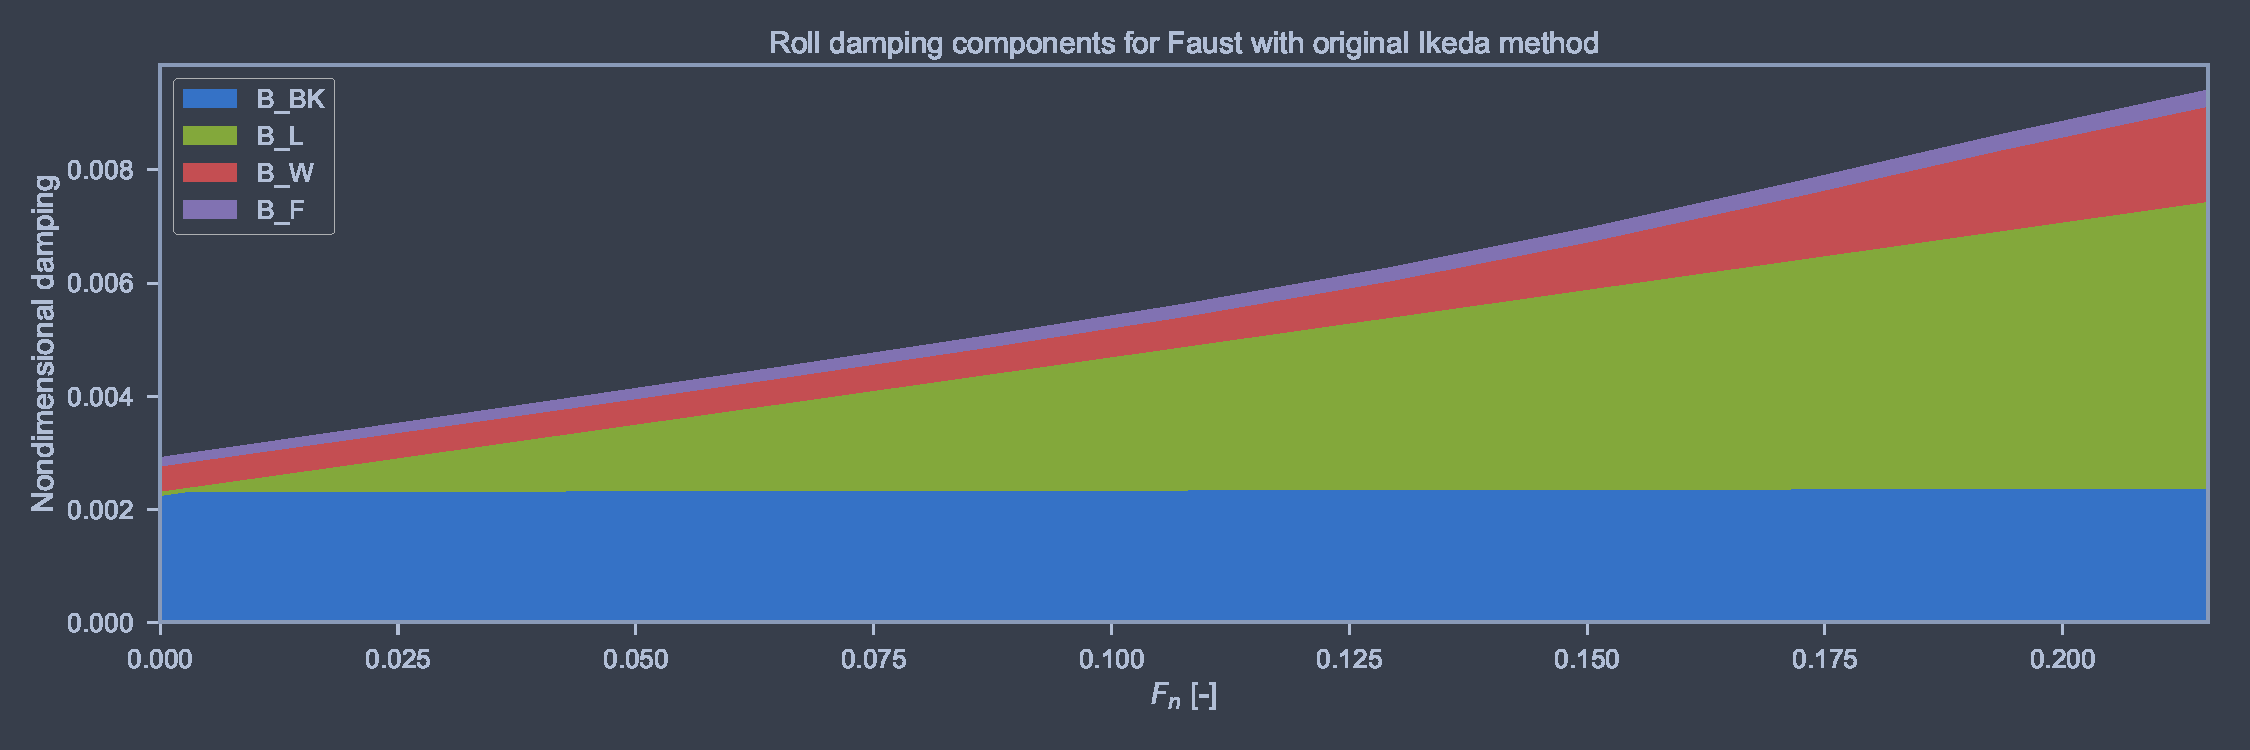
\includegraphics[width=\columnwidth]{figures/ikeda_faust.pdf}
    \caption{Roll damping components calculated with Ikeda method for PCTC Faust}
    \label{fig:ikeda_faust}
\end{figure}



Ikedas original method require strip method calculations. This is not an attractive option for the present study since that would require calculations with exact hull geometries to be carried out for all of the ships in the study. There exist however a \emph{Simplified Ikeda method} \cite{kawahara_simple_2011} that is instead used in this study \emph{Simplified Ikeda method} predicts the roll damping components at zero speed.

A study of the has been conducted which shows the roll damping components for various speeds. Calculations with *Ikeda original method* and the *Simplified method* have been carried for two ships (*S175* and *Faust*). The two methods show reasonable agreement for zero speed.

In order to introduce a speed dependancy to the *Simplified method* the following is conducted:
* Add Lift damping $B_L$.
* Add speed dependence of wave damping $\frac{B_W}{B_{W0}}$
* Remove $B_E$ at ($F_n>0.15$) ?
\section{Accuracy of current methods for predicting roll damping}
\label{se:accuracy_SI_method}
It was shown by \parencite{kawahara_simple_2011} that Ikeda's method does not work for some modern ships with buttock flow sterns. \parencite{soder_assessment_2019} also showed that Ikeda's method was not capable of accurately predicting the roll damping for a Pure Car and Truck Carrier. The SI-method being a simplified version of Ikeda's method most likely inherits its problems but also introduces some extrapolation errors as reported by \parencite{rudakovic_application_2017}. In the following, 227 existing roll decay model tests conducted at SSPA Maritime Dynamics Laboratory are used to validate the SI-method. The comparison will help identify the drawbacks and improvement potentials of the SI-method. It aims at further developing this method to increase its accuracy through some statistical regression analysis based on the large test database.

\subsection{Overall accuracy of Simplified Ikeda method}
\label{se:overall_comparison}
%An investigation of how well the implementation of the SI-method agrees with the corresponding results in the roll damping database has been carried out. 
Comparing roll damping is a bit difficult since the roll damping model consist of two coefficients, a linear term $B_1$ and a quadratic term $B_2$. These coefficients can be combined by calculating the equivalent damping coefficient for a certain roll angle $\phi_a$ \parencite{himeno_prediction_1981}:

\begin{equation}
B_{e} = B_{1} + \frac{8 B_{2} \omega_{0} \phi_{a}}{3 \pi}
\end{equation}


For the roll damping database $B_1$ and $B_2$ can be inserted directly into Eq.(\ref{eq:B_e_equation}) to get the equivalent roll damping $B_e$. In order to obtain the same coefficients for the SI-method, roll damping was calculated for two roll amplitudes $\phi_a$ for the same motion frequency. $B_1$ and $B_2$ are obtained by fitting the Eq.(\ref{eq:B_e_equation}) to this data \parencite{himeno_prediction_1981}. The $B_e$ coefficient was made non-dimensional according to \parencite{himeno_prediction_1981}  giving the non-dimensional equivalent linear damping coefficient $\hat{B_e}$, which was more convenient to use for this comparison as follows,
\begin{equation} \label{eq:be_eqvalent}
    \hat{B_e} = \frac{B_e}{\rho \bigtriangledown Beam^2} \sqrt{\frac{Beam}{2g}},
\end{equation}
where $\rho$, $\bigtriangledown$ and $Beam$ stand for fluid density, displacement volume and breadth of a ship, respectively.
For the roll decay tests at SSPA, i.e., the database used in this study, the initial roll angle is normally set to 10 degrees, so that the model test data contain amplitudes in the range between 0 and 10 degrees. The root mean squared error of the equivalent roll damping, $RMSE_{\hat{B}_e}$, for various initial roll angles $\hat{B}_e(\phi_a)$ between estimation by the SI-method and the model test results is,

\begin{equation} \label{eq:rmse}
    RMSE({\hat{B}_e} (\phi_a)) = \sqrt{\frac{\sum\limits_{i=1}^n (\hat{B}_{e,i}^{SI} (\phi_a) - \hat{B}_{e,i}^{model} (\phi_a))^2}{n}},
\end{equation}
where $\hat{B}_{e,i}^{SI} (\phi_a)$ represents the equivalent roll damping by the SI-method for the i-th model test with initial roll angle of $\phi_a$, while $\hat{B}_{e,i}^{model} (\phi_a)$ represents the damping from the model tests. The results of the RMSE are plotted in the upper plot of Fig.\ref{fig:ikeda_phi_a}. Large values of $RMSE({\hat{B}_e})$ indicate very bad agreement between the SI-method and the model test results for roll damping prediction of modern ships. It should be noted that the accuracy decrease for larger amplitudes where nonlinear part of the SI-method plays a larger part. Furthermore, in order to illustrate the difference of $\hat{B}_e$ prediction between the SI-method and the model tests at SSPA, the three bottom plots of Fig.\ref{fig:ikeda_phi_a} presents the comparison for three roll amplitudes $\phi_a$ equal to 0, 5, 10 degrees, respectively. It shows that the accuracy differ very much between the amplitudes, with the highest accuracy at zero roll amplitude. 


\begin{figure}[H]
\centering
  \centering
  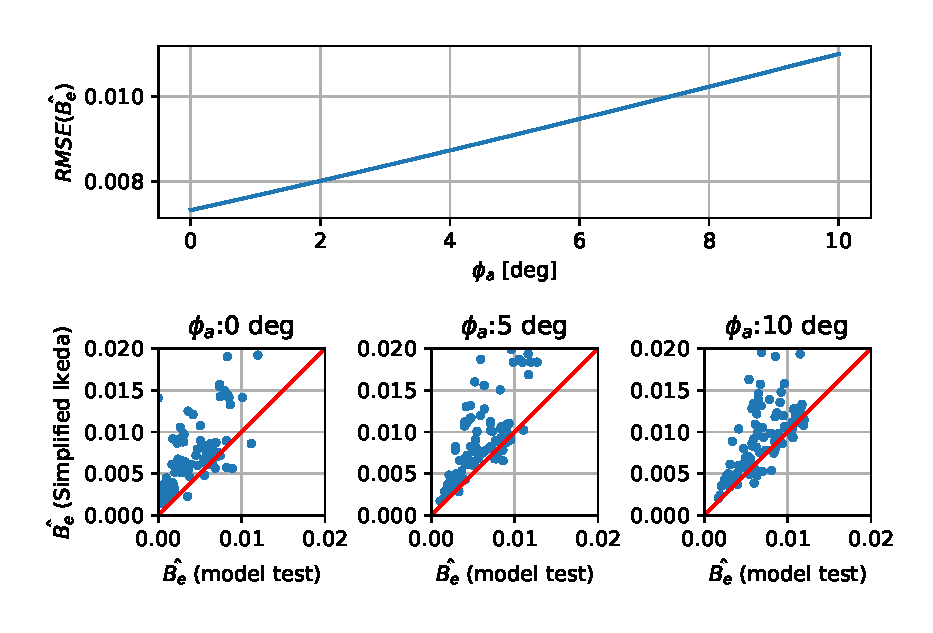
\includegraphics[]{figures/ikeda_phi_a.eps}
  \vspace{-0.5cm}
  \caption{Root mean square error of roll damping prediction between the SI-method and the model test results (upper plot). Influence of roll amplitude $\phi_a$ on $\hat{B_e}$ between the SI-method and model tests for $0^{\circ}$ (bottom left plot), $5^{\circ}$ (bottom middle plot) and $10^{\circ}$ (bottom right plot), respectively.}
  \label{fig:ikeda_phi_a}
\end{figure}

It was found that almost all ships in the roll damping database were outside the limits that are suitable to be applied in Eq.(\ref{eq:SI_limits}). Two different ways to handle this limit exceedance was investigated:
\begin{enumerate}
  \item the ``unlimited" approach where the input values are allowed to exceed the limits.
  \item the ``limited" approach where the limit boundary values were used for exceeding values.
\end{enumerate}

Fig.\ref{fig:ikeda_limited} show the comparison of roll damping predictions by the SI-method at 2 degrees roll amplitude, using the ``unlimited" and ``limited" approach with the corresponding results from model tests. The ``limited" approach seems to be the best one to use according to this figure, where the ``unlimited" approach has values very far away from the model test results (far away from the red reference line).   


\begin{figure}[H]
\vspace{-0.5cm}
\centering
  \centering
  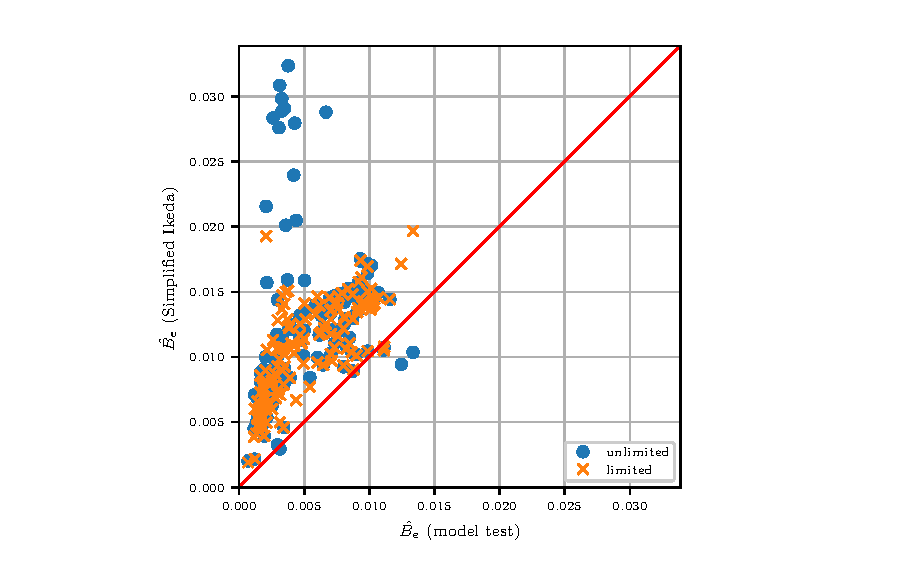
\includegraphics[]{figures/ikeda_limited.eps}
  \vspace{-0.5cm}
  \caption{$\hat{B_e}$ at all speeds estimated by the simplified Ikeda's method (Y-axis) in comparison with that from the roll decay test database (X-axis)}
  \label{fig:ikeda_limited}
\end{figure}


\subsection{Sensitive analysis of SI methods for the ship data}
\label{se:accuracy_SI_method}
Prior to the validation the behaviour of the SI-method was studied by varying the input parameters between minimum and maximum values in database around a point "reference ship" with values in the middle of the input boundaries (Eq. \ref{eq:SI_limits}) (see figure \ref{fig:SI_sensitivity}). It can be seen that the wave damping $B_W$ increases a lot with the absolute value of $OG/T$. It can also be seen the the wave damping has an enormous increase when the beam to draught ratio exceeds the input boundary, which seems to be the case for at least one third of the roll decay tests. It can also be noted that most of the ships in the database have midsection coefficients $A_0$ and bilge keel heights outside the limits. 

\begin{figure}[H]
    \centering
    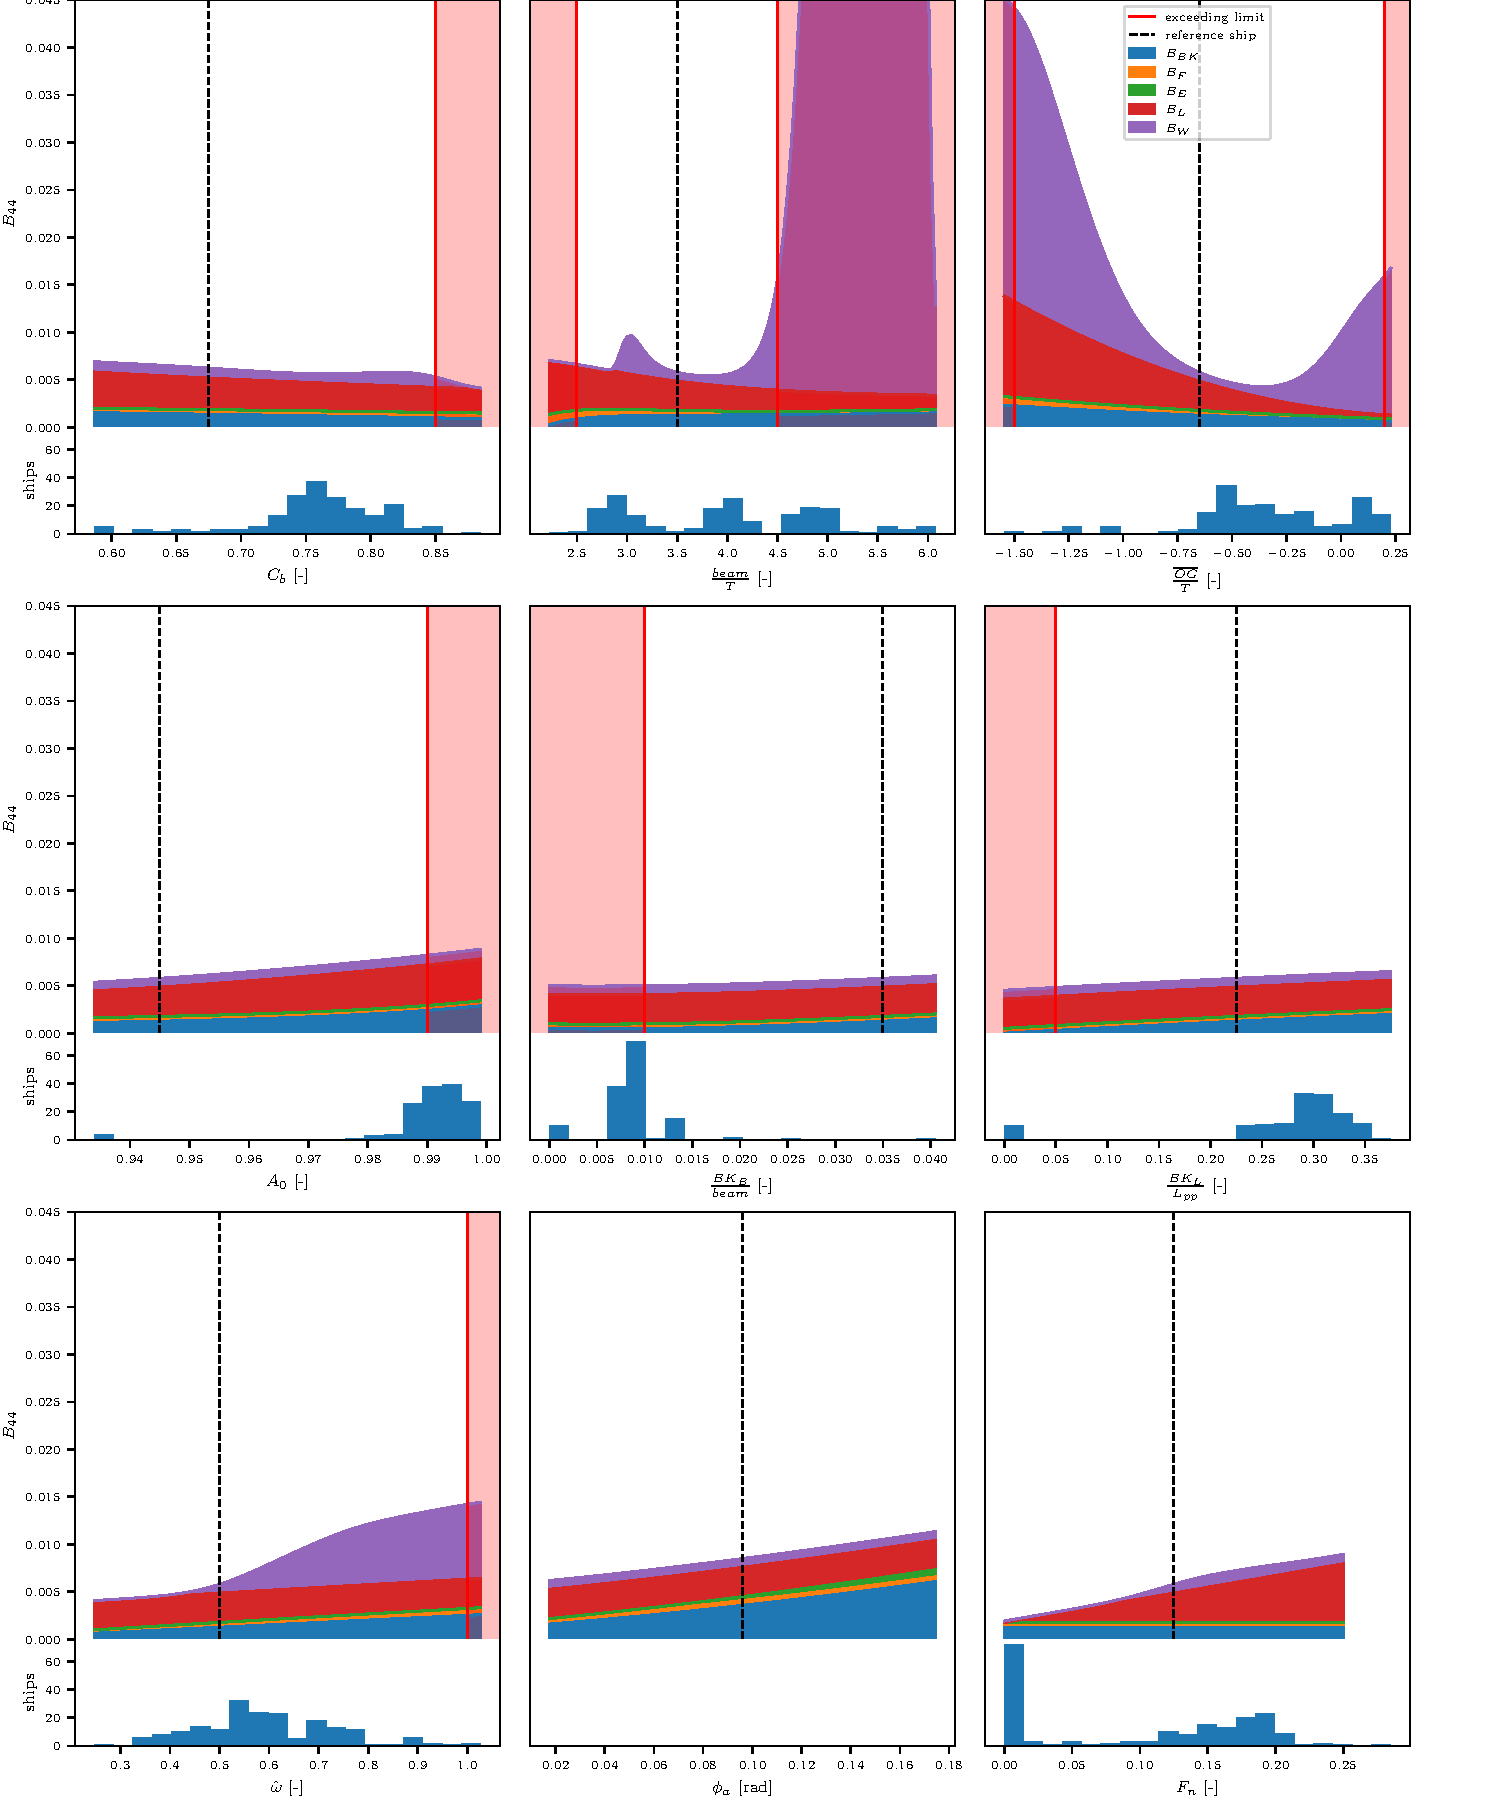
\includegraphics[width=\textwidth]{figures/SI-sensitivity.pdf}
        \vspace{-0.5cm}
    \caption{SI-method input parameter variation and data base ships}
    \label{fig:SI_sensitivity}
\end{figure}


\subsection{Simplified and original Ikeda method}
\label{se:si_ikeda_model}
Since the agreement between the SI-method and the reference model test result was not very good a second study was conducted to see if the original Ikeda method would give better results. In the Ikeda method more detailed information about the ship hull geometry is needed so that $B_W$ can be calculated with a strip method and $B_E$ can be calculated using sectional lewis coefficients. It was possible to collect the required hull inputs for 14 ships in the database. Scale models of these ships were used in 46 of the reference roll decay tests.

\begin{figure}[H]
    \centering
    \includegraphics[width=6in, height = 8in ]{figures/si_}
        \vspace{-0.5cm}
    \caption{SI-method input parameter variation and data base ships}
    \label{fig:s}
\end{figure}

\section{Simplified Ikeda method}
\label{se:simplified_ikeda}
The \emph{Simplified Ikeda method} \cite{kawahara_simple_2011} has been implemented with the intention to be used both as a benchmark and maybe also as a sub-component of a new method. The examples from \cite{kawahara_simple_2011} was recalculated to check that the method has been implemented correctly.

Both  \emph{Simplified Ikeda method} can

The equivalent linear damping coefficient 
\begin{equation}
B_{e} = B_{1} + \frac{8 B_{2} \omega_{0} \phi_{a}}{3 \pi}
\end{equation}


\section{Results}
\label{se:results}

\begin{itemize}
  \item A roll decay database with 400 roll decay tests has been created.
  \item A roll damping database has been build with roll damping coefficients from system identification of roll decay tests.
  \item A classification of the roll damping results has been conducted.
  \item The accuracy of Ikedas simplified method has been investigated by benchmark with roll damping database.
  \item A new method has been proposed, based on regression of the roll damping database, as an improvement to the simplified Ikeda method.
\end{itemize}


\section{Conclusions}
\label{se:conclusions}
The roll damping database has been compared with predictions with the implementation of the Simplified Ikeda method. The database and the predictions show agreement for some cases but poor agreement for other cases, especially for small draft to beam ratios, typically for Ballast loading condition for many modern ships. It seems that exceeding the limits of the the Simplified Ikeda method will give poor results. These limits are unfortunately not so well defined in \parencite{kawahara_simple_2011}. The comparison in the present paper suggest a lower limit of the draught to length ratio of $T/L_{pp}>0.034$.

A regression model has been developed which has better accuracy than the Simplified method for the present roll damping data. The accuracy of the regression model has been investigated using extensive cross validation. The model should be able to predict the roll damping for ships with main dimensions similar to the once in this paper within the estimated accuracy.
If higher accuracy is needed, more advanced methods can be used, such as the original Ikeda method with strip calculations, CFD or model testing, to get reliable roll damping predictions.

\section{Discussion}
The test setup in the free roll decay tests differs from the forced roll motion model tests that Ikeda \parencite{ikeda_velocity_1979} used to derive the original method. This is not believed to have any large impact as long as roll damping near the natural frequency is considered. The Ikeda model tests were also conducted with smaller models (2 meters compared to 3-6 meters). But there is a skin friction component $B_F$ to the Ikeda method that should handle this scale effect.



\section*{Acknowledgements}
\label{se:acknowledgements}
The authors would like to acknowledge Trafikverket (Swedish Transport Administration) and Lighthouse for providing the resources to prepare this paper and also thank all personnel at SSPA that have been involved in the creation of the model test results: building the ship models and conducting the experiments. Also special thanks to Sune Thorsson who collected the meta data about the tested ship models.





\section{References}
\label{sec:references}

\bibliographystyle{unsrt}
%\bibliographystyle{abbrvnat}
\bibliography{references}


\end{document}
